\subsection{Servo}
On the vehicle there is a servo, which is a S3003 by Futaba. \todo{Insert ref to the datasheet}
The servo is used for the steering of the vehicle. The way the servo turn the vehicle, is by braking the gears (part 3 on \figref{vehicleDescriptionDriveTrain} in \secref{sec:Vehicledescription}) in one side, and transfer that power over to the other side. The transfer of power is done by the differential gear box, which is explained in \secref{sec:Differentialgears}.

The Servo is controlled by a PWM signal from a controller. The received PWM signal is converted into an angle by the servo and will affect the position of the mechanical arm, mounted on the servo. The mechanical arm is connected to two brakes, one for each gear, that the servo is set to brake on. When the arm is rotated one way, it triggers the brakes in that side, the arm rotated to. The other side is not affected, when the servo is braking on first side. The arm rotated according to the value of the angle, it gets through the PWM signal (See \figref{timeVSangle}).

\begin{figure}[H]
	\centering
	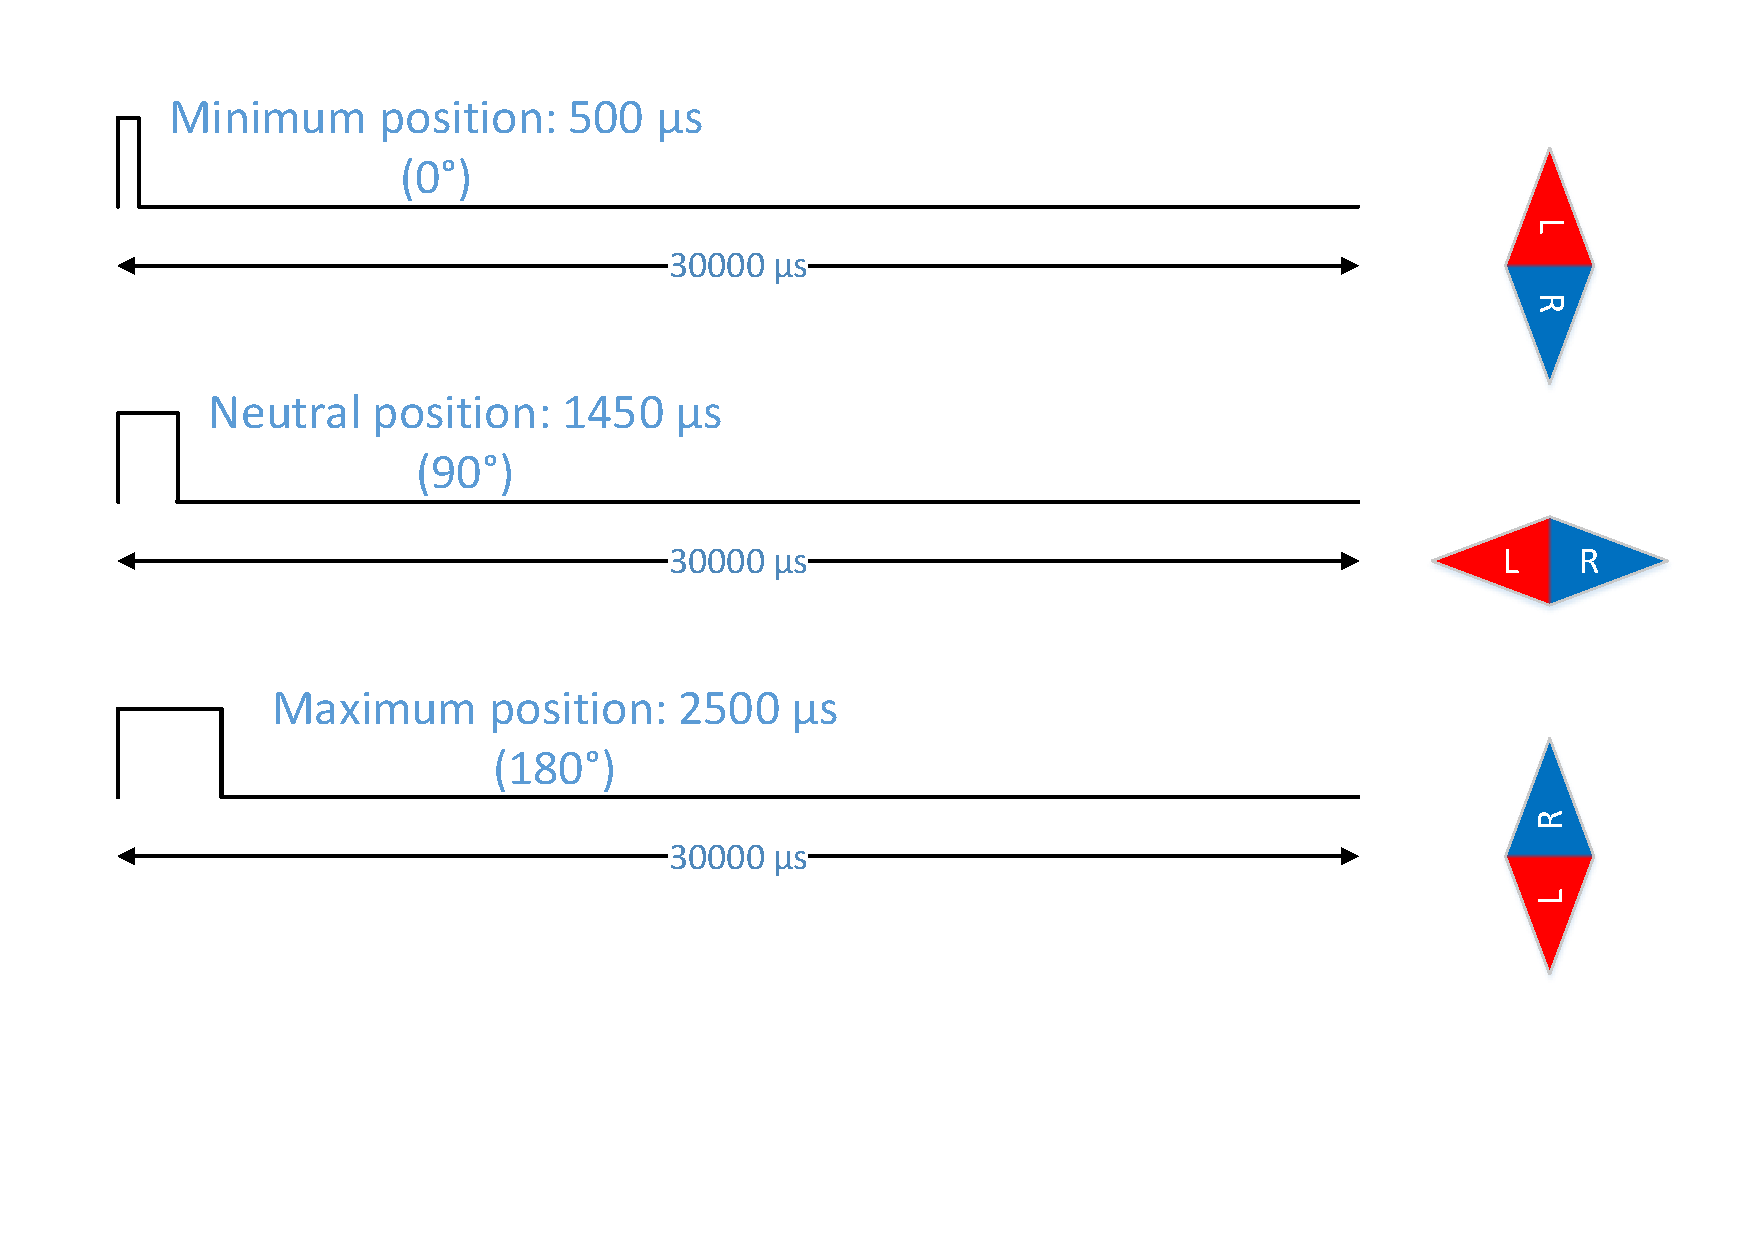
\includegraphics[scale=0.6]{figures/TimeVSangle.pdf}
	\caption{Convertion from PWM to angle by the servo. The figure to the right, show how the mechanical arm reacts to the PWM signal (Blue is right side of the arm and red is left side). The minimum position is defined as 0°, neutral position is defined as 90° and maximum position is defined as 180°.}
	\label{timeVSangle}
\end{figure}

The servo reacts linearly to the PWM signal and the cycle of the signal is 30000 mikroseconds \todo{Insert ref to the datasheet}. The indication of the which angle the arm is having, is made from the minimum position. This is because it is the angle that the arm have with the smallest PWM signal, the servo can use. This position is set to 0°.
 
 When the mechanical arm is in neutral position, it is in a position, where none of the gears is effected by a braking force. This position is indicated as 90°, as it is turned a quarter of a turn from the minimum position. When the angle is smaller than 90°, the servo will trigger the right brake and begin to slow down the right gear. This position of the arm will not effect the left brake. When the angle is bigger than 90°, the reverse function will happen and the left brake is triggered and the right brake will not be braking the gear.

When the servo brakes on one of the belt, the force, that should be lost in the braking, is transfer to the other belt, by the differential gear system.